\subsection{Introduction}

\subsubsection{Inspiration}

Following on from the library of compounds based on \textit{P. aeruginosa} autoinducers, a series of conjugates based on \textit{analogues} of C$_4$-HSL were planned. This strategy was inspired by a paper\cite{Ganguly2011} and patent\cite{Iyer2012} by Ganguly \textit{et al.}, who synthesised and characterised a conjugate \compound{cmpd:SHL4CipMe} of methyl ciprofloxacin with homocysteine thiolactone (see \ref{fig:SHL4CipMe}). Homocysteine thiolactone is an analogue of homoserine lactone with the ring oxygen replaced by sulfur, and has been used as the head group in several other known quorum sensing modulators\cite{Eberhard1986,Schaefer1996,Passador1996,Smith2003,Chhabra1993,McInnis2011,Geske2007,Janssens2007}.\todo{show compounds it's in and describe?}

\begin{figure}[H]
	\begin{center}
		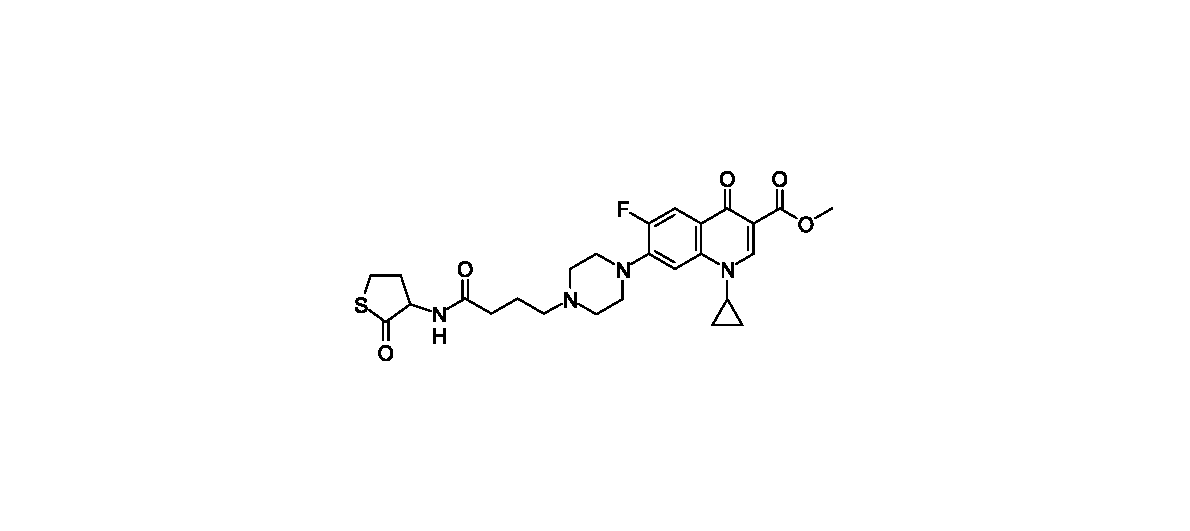
\includegraphics[scale=1]{SHL4CipMe}
		\caption{The HCTL-CipMe conjugate \compound{cmpd:SHL4CipMe} studied by Ganguly \textit{et al.}\cite{Ganguly2011,Iyer2012}.\label{fig:SHL4CipMe}}
	\end{center}
\end{figure}


As part of their characterisation of the HCTL-CipMe conjugate \compound{cmpd:SHL4CipMe}, Ganguly \textit{et al.} found the minimum inhibitory concentration (MIC) of the conjugate in \textit{P. aeruginosa} under standard planktonic conditions. 
The MIC was found to be ten times higher for the conjugate vs. ciprofloxacin (50 vs. 5 $\mu$m), indicating that the conjgate was less effective than ciprofloxacin under planktonic conditions. 

Ganguly \textit{et al.} then investigated the effect of the conjugate on biofilms. 
The conjugate and ciprofloxacin were first added to dilute \textit{P. aeruginosa} liquid culture at 25 $\mu$m. 
As expected, the culture failed to grow and form biofilm in the presence of ciprofloxacin, but did grow in the presence of the conjugate \compound{cmpd:SHL4CipMe}. 
They then incubated cultures for 24 h, to allow biofilms to grow, before adding the compounds. In contrast, they found that the conjugate \compound{cmpd:SHL4CipMe} disrupted the biofilm more effectively than ciprofloxacin. 
When the biofilm was grown for 48 or 72 hours the conjugate had similarly disruptive effects, whereas ciprofloxacin `did not show any significant antibacterial activity'.

These results are exciting as they hint that an autoinducer conjugate might be able to combat an established \textit{P. aeruginosa} infection more effectively than the unmodified antibiotic. 
Ganguly \textit{et al.} suggest that their conjugate is more effective than ciprofloxacin in penetrating biofilms, and/or better at avoiding being pumped out by multidrug efflux pumps. They posit that this could be due to the thiolactone head, as they also showed that unconjugated C$_4$-HCTL \compound{cmpd:SHL4} (see \ref{fig:HL_SHL}) has `either enhanced uptake or functional activity' when compared with C$_4$-HSL \compound{cmpd:HL4}. 

\begin{figure}[H]
	\begin{center}
		\schemeref[HL4]{cmpd:HL4}
		\schemeref[SHL4]{cmpd:SHL4}
		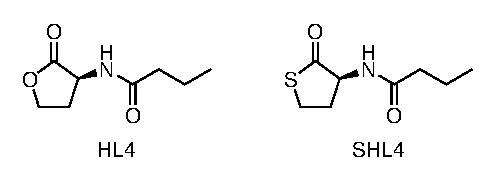
\includegraphics[scale=1]{HL_SHL}
		\caption{
		C$_4$-HSL \compound{cmpd:HL4} and C$_4$-HCTL \compound{cmpd:SHL4}. Note that Ganguly \textit{et al.} tested the \textit{S} enantiomer of C$_4$-HCTL \compound{cmpd:SHL4}, but used a racemic mixture in their HCTL-CipMe conjugate.
		\label{fig:HL_SHL}}
	\end{center}
\end{figure}

While the results found by Ganguly \textit{et al.} show promise, they only test one conjugate, and do not include controls to show that the HCTL group specifically is necessary for the enhanced effect.
It was therefore decided to build on this work by synthesising a series of ciprofloxacin conjugates with head groups known as part of quorum sensing modulators\cite{Galloway2011,Hodgkinson2012a}.\todo{read these again, put ones I didn't do in further work}

%The formation of biofilms can drastically increase MIC for many antibiotics \cite{Ceri1999}. For ciprofloxacin in \textit{P. aeruginosa} the MIC increases by 16 fold according to Ceri \textit{et al.} 

%Ganguly \textit{et al.} used Bac-Light Live/Dead staining and confocal microscopy to image the biofilms, whereas so far I have used crystal violet staining. Crystal violet does not differentiate between live or dead cells, and so might not pick up on the antibacterial effects of compounds. However, their confocal microscopy results show a quantifiable decrease in biofilm thickness, and it may be possible to detect this using crystal violet.

%Is it just more lipophillic?



\subsubsection{Head groups}

The activity of the chosen head groups against \textit{P. aeruginosa} receptors when coupled with the native C$_4$ and 3-oxo-C$_12$ tails is summarised in \ref{tbl:head_groups}. It is hoped that high activity of these molecules should correlate with high activity of their ciprofloxacin conjugates.
This is not a comprehensive list of active head groups, and other possible choices are covered in \ref{sec:future}.

The exact head groups used in this study are shown in \ref{fig:head_groups}. The cyclohexanol derivatives were synthesised as a diastereomerically pure racemate, whereas the cyclopentanol derivatives were synthesised as separate enantiomers. Unfortuantely, cyclopentanone derivatives were not synthesised, and would be an obvious future addition to the library. The 2-methoxybenzene derivatives do not have precedents as quorum sensing modulators in the literature, but they were included so as to be compared with the 3-methoxybenzene derivatives.

\todo{check Boursier2018 for print publication details}

\begin{table}[H]
  \centering
\begin{tabular}{|P{0.18\textwidth}|p{0.32\textwidth}|p{0.32\textwidth}|}
\hline 
 \vspace{8px}\textbf{Head group} & \vspace{0px}\centering
\includegraphics[scale=1]{C4_tail} & \centering\arraybackslash\vspace{0px}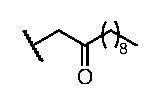
\includegraphics[scale=1]{oddhl_tail} \\ 
\hline 
 \vspace{0px}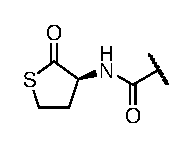
\includegraphics[scale=1]{SHL_head} & Partial agonist and antagonist against LasR\cite{McInnis2011}. Shown to increase biofilm formation in \textit{P. aeruginosa}\cite{Ganguly2011}.
 & Strong agonist against LasR, with comparable activity to the native ligand\cite{Smith2003,Boursier2018,Passador1996,McInnis2011}. \\ 
 %L vs racemate doesn't matter \cite{McInnis2011} D might actually do better?
 %check receptor. hydrolytic stability is higher for SHL. is it racemic in Ganguly?
 %Some evidence that \textit{R} enantiomer is more potent\cite{McInnis2011}.
%\hline 
% \vspace{0px}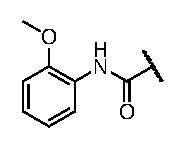
\includegraphics[scale=1]{2MeOA_head} 
% & Not yet studied. 
% & Not yet studied. \\  
\hline 
 \vspace{0px}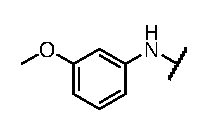
\includegraphics[scale=1]{3MeOA_head} 
 & Partial agonist against LasR\cite{Hodgkinson2012a}. 
 & Strong antagonist against LasR\cite{Hodgkinson2012a}. \\ 
\hline 
 \vspace{0px}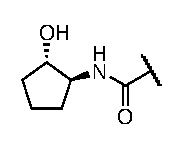
\includegraphics[scale=1]{HOcy5_S_head} 
 & Poor agonist and antagonist against RhlR\cite{Smith2003a,Jog2006}.
 & Strong antagonist against LasR\cite{Smith2003a}.\\ 
\hline 
 \vspace{0px}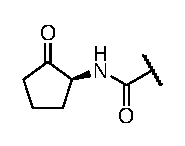
\includegraphics[scale=1]{Ocy5_S_head} 
 & Strong agonist against RhlR\cite{Smith2003a}. \textit{SS} enantiomer is more potent\cite{Jog2006}.
 & Partial agonist against LasR\cite{Smith2003a}. \\ 
\hline 
 \vspace{0px}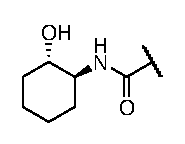
\includegraphics[scale=1]{HOcy6_S_head} 
 & Strong agonist against RhlR\cite{Smith2003a}. \textit{SS} enantiomer is more potent, with comparable activity to the native ligand\cite{Jog2006}.
 & Strong agonist against LasR\cite{Smith2003,Smith2003a}. \textit{SS} enantiomer is more potent, with comparable activity to the native ligand\cite{Jog2006}.\\ 
\hline 
 \vspace{0px}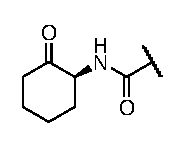
\includegraphics[scale=1]{Ocy6_S_head} 
 & Strong agonist against RhlR\cite{Smith2003a}. \textit{SS} enantiomer is more potent\cite{Jog2006}.
 & Partial antagonist against LasR\cite{Smith2003a}. Shown to reduce biofilm formation in \textit{P. aeruginosa}\cite{Smith2003a}.\\ 
\hline 
\end{tabular}
\caption{Activities of autoinducers containing the chosen head groups when coupled with C$_4$ or 3-oxo-C$_12$ tails.\label{tbl:head_groups}} 
\end{table}

\begin{figure}[H]
	\begin{center}
		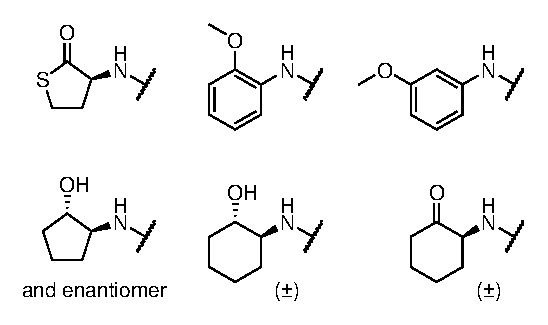
\includegraphics[scale=1]{head_groups}
		\caption{The head groups used in this section.\label{fig:head_groups}}
	\end{center}
\end{figure}

\subsubsection{Linkers}

As Ganguly \textit{et al.}\cite{Ganguly2001} synthesised their conjugate from Br-C$_4$-HCTL, it was envisaged that a branching strategy could be used to produce two sets of conjugates (see \ref{sch:branching_synth_general}). The first set would be formed by the S$_N$2 reaction of the relevant bromide with methyl ciprofloxacin. The second set would be made by displacing the bromide with azide, then performing a click reaction with the alkynyl ciprofloxacin derivative \compound{cmpd:Y4Cip} made previously to form the triazole-linked product. Ketone conjugates would be formed by oxidation of the alcohols.

\begin{scheme}[H]
	\begin{center}
		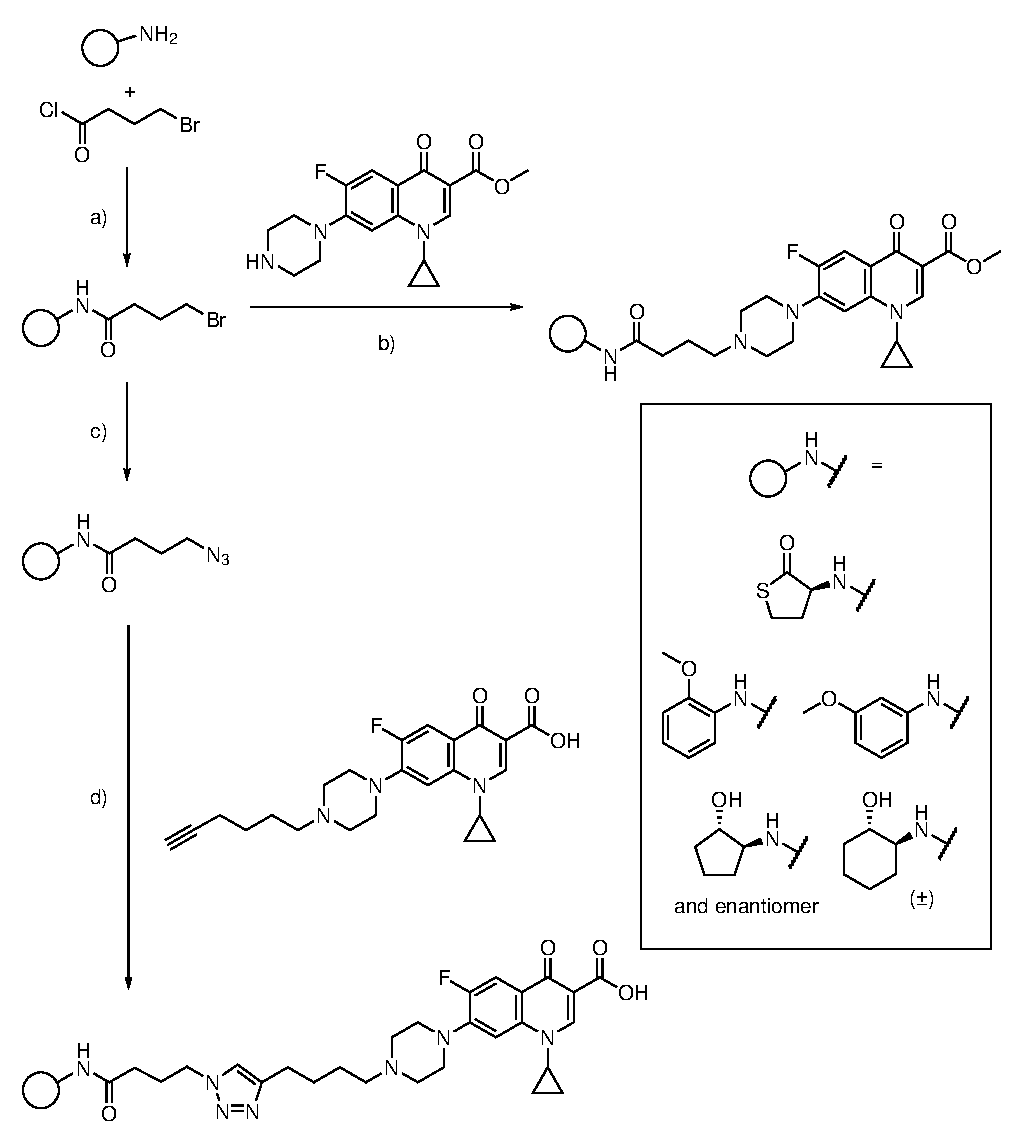
\includegraphics[scale=1]{branching_synth_general}
		\caption{\label{sch:branching_synth_general}}
	\end{center}
\end{scheme}

\subsection{Homocysteine thiolactone derivatives\label{sec:HCTL}}

\subsubsection{Synthesis of methyl ciprofloxacin \compound{cmpd:CipMe}}

The synthesis of the analogue conjugates began with the synthesis of methyl ciprofloxacin \compound{cmpd:CipMe}, which would then be attached to the various head groups.
Methyl ciprofloxacin \compound{cmpd:CipMe} was synthesised from ciprofloxacin \compound{cmpd:Cip} and MeOH in very good yield using \textit{para}-toluenesulfonic acid as a catalyst \cite{Sachin2010}.

\begin{scheme}[H]
	\begin{center}
		\schemeref[Cip]{cmpd:Cip}	
		\schemeref[CipMe]{cmpd:CipMe}
		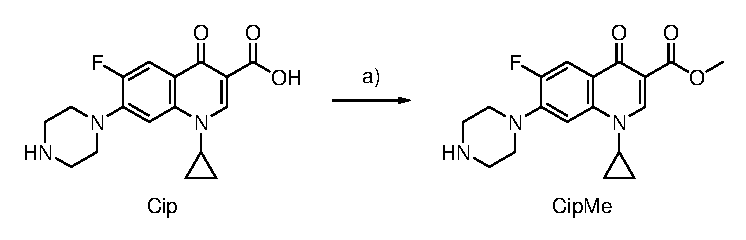
\includegraphics[scale=1]{CipMe_synth}
		\caption{Synthesis of methyl ciprofloxacin \compound{cmpd:CipMe}. a) \textit{p}-TSA, MeOH, 72 h, reflux, 83.3 \%. \label{sch:CipMe_synth}}
	\end{center}
\end{scheme}

\subsubsection{Synthesis of Br-C$_4$-HCTL \compound{cmpd:SHL4Br}}

The HCTL head group was then attached to the linker to form Br-C$_4$-HCTL \compound{cmpd:SHL4Br}, in preparation for coupling to methyl ciprofloxacin \compound{cmpd:CipMe}.
Br-C$_4$-HCTL \compound{cmpd:SHL4Br} was synthesised using the Schotten-Baumann conditions employed previously for the HSL derivatives \compound{cmpd:HL4Br} and \compound{cmpd:HL6Br}. Br-C$_4$-HCTL \compound{cmpd:SHL4Br} was isolated in markedly higher yield than that achieved by Ganguly \textit{et al.}\cite{Ganguly2011} (87.9 \% vs. 25.0 \%). It is possible that this was due to \ce{CH2Cl2} being used for the extraction, whereas Ganguly \textit{et al.} used EtOAc.

\begin{scheme}[H]
	\begin{center}
		\schemeref[Cl4Br]{cmpd:Cl4Br}
		\schemeref[SHLHCl]{cmpd:SHLHCl}	
		\schemeref[SHL4Br]{cmpd:SHL4Br}
		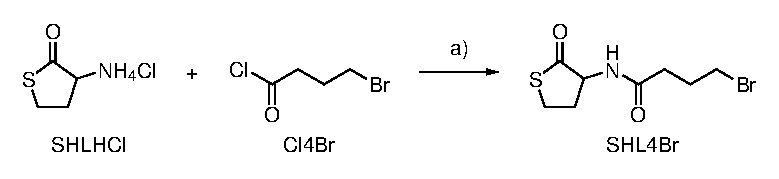
\includegraphics[scale=1]{SHL4Br_synth}
		\caption{Synthesis of Br-C$_4$-HCTL \compound{cmpd:SHL4Br}. a) \ce{NaHCO3}, \ce{CH2Cl2}, \ce{H2O}, 0 $^{\circ}$C, 1 h, 87.9 \%.\label{sch:SHL4Br_synth}}
	\end{center}
\end{scheme}

\subsubsection{Synthesis of the HCTL-CipMe conjugate \compound{cmpd:SHL4CipMe}}

The HCTL-CipMe conjugate \compound{cmpd:SHL4CipMe} was synthesised using the procedure outlined by Ganguly \textit{et al.}\cite{Ganguly2011}. Monitoring by LCMS showed slow conversion to the product. Br-C$_4$-HCTL \compound{cmpd:SHL4Br} was presumably consumed by side reactions as 4 eq. were required to reach full conversion. Ganguly \textit{et al.} do not quote a yield for comparison\cite{Ganguly2011,Iyer2012}, but it is hoped that the 12.2 \% achieved here could be improved upon. The side reactions led to the production of an unidentified brown, viscous contaminant which made purification by flash column chromatography (as was used by Ganguly \textit{et al.}) challenging. Preparatory HPLC on a partially purified sample gave enough pure HCTL-CipMe conjugate \compound{cmpd:SHL4CipMe} for biological testing. 

Future optimisation of the synthesis could focus on different routes to the product, e.g. the peptide coupling described in \ref{sec:CipMe_linker}, or different purification methods, e.g. using just preparatory HPLC, or reverse phase flash column chromatography.

\begin{scheme}[H]
	\begin{center}
		\schemeref[CipMe]{cmpd:CipMe}
		\schemeref[SHL4CipMe]{cmpd:SHL4CipMe}
		\schemeref[SHL4Br]{cmpd:SHL4Br}
		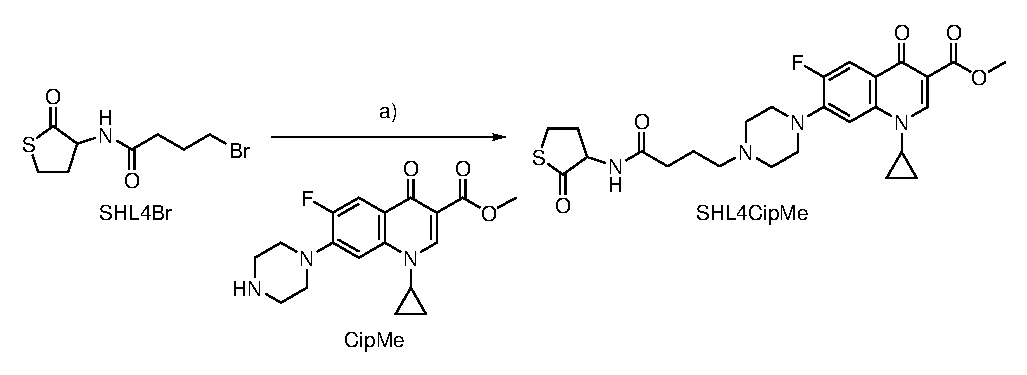
\includegraphics[scale=1]{SHL4CipMe_synth}
		\caption{
			Synthesis of the HCTL-CipMe conjugate \compound{cmpd:SHL4CipMe}, 
			\ce{N3}-C$_4$-HCTL \compound{cmpd:SHL4N3}, and
			the HCTL-Cip triazole conjugate \compound{cmpd:SHL4T4Cip}.
			a) \ce{K2CO3}, acetonitrile, reflux, 24 h, 12.2 \%.
			\label{sch:SHL4CipMe_synth}}
	\end{center}
\end{scheme}

\subsubsection{Synthesis of the HCTL-Cip triazole conjugate \compound{cmpd:SHL4T4Cip}}

Br-C$_4$-HCTL \compound{cmpd:SHL4Br} was converted into \ce{N3}-C$_4$-HCTL \compound{cmpd:SHL4N3} (see \ref{sch:SHL4CipMe_synth}), by an S$_N$2 reaction with sodium azide which proceeded in excellent yield. 

\ce{N3}-C$_4$-HCTL \compound{cmpd:SHL4N3} was then subjected to the click reaction conditions optimised previously (see \ref{sec:click_general}). The reaction proceeded very slowly at first, until it was realised that the azide did not dissolve in the reaction solvent and formed a single solid clump. DMSO was added as a co-solvent, and the reaction began to proceed, albeit still slowly. It is possible that the sulfur atom coordinates to the copper, thus inhibiting its catalytic ability. Nonetheless the HCTL-Cip triazole conjugate \compound{cmpd:SHL4T4Cip} was eventually isolated in good yield (see \ref{sch:SHL4T4Cip_synth}).

\begin{scheme}[H]
	\begin{center}
		\schemeref[SHL4Br]{cmpd:SHL4Br}
		\schemeref[SHL4N3]{cmpd:SHL4N3}
		\schemeref[Y4Cip]{cmpd:Y4Cip}
		\schemeref[SHL4T4Cip]{cmpd:SHL4T4Cip}
		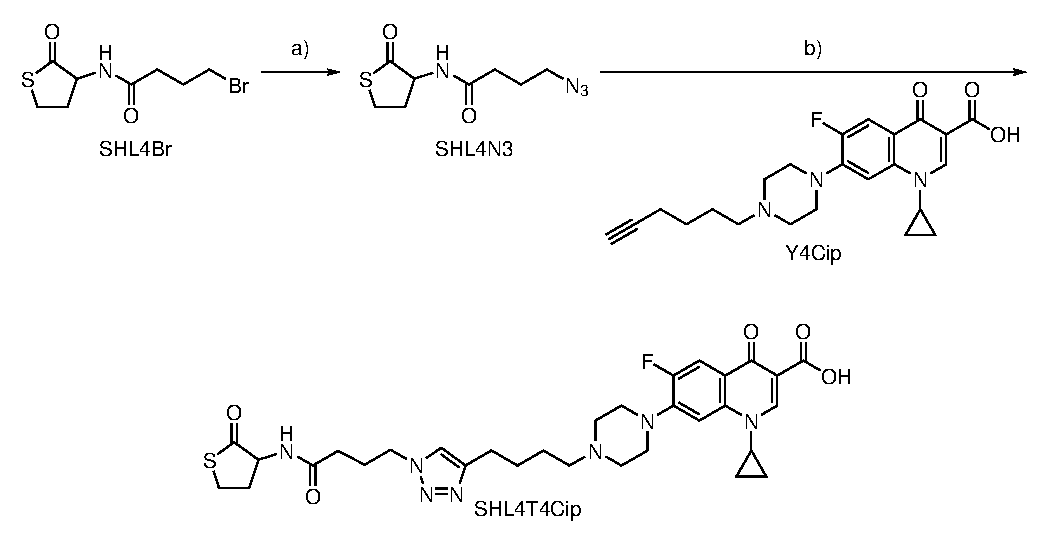
\includegraphics[scale=1]{SHL4T4Cip_synth}
		\caption{
			Synthesis of the HCTL-Cip triazole conjugate \compound{cmpd:SHL4T4Cip}.
			a) \ce{NaN3}, acetonitrile, reflux, 1.5 h, 89.3 \%.
			b) \ce{CuSO4}, THPTA, sodium ascorbate, \ce{H2O}, \textit{t}-BuOH, DMSO, r.t., 7 d, 70.6 \%.
			\label{sch:SHL4T4Cip_synth}}
	\end{center}
\end{scheme}

\subsubsection{Synthesis of the cleavable HCTL-Cip triazole conjugate \compound{cmpd:SHL4THCip}}

A cleavable conjugate \compound{cmpd:SHL4THCip} was also synthesised from \ce{N3}-C$_4$-HCTL \compound{cmpd:SHL4N3} by reaction with a cleavable alkyne-Cip derivative \compound{cmpd:Y4HCip} synthesised previously by Prof. Eddy Sotelo-Perez (see \ref{sec:cleavable}). Conditions developed by Prof. Sotelo-Perez were used, but again the reaction proceeded very slowly. The disappointing yield is, however, most likely due to losses during purification.

\begin{scheme}[H]
	\begin{center}
		\schemeref[SHL4N3]{cmpd:SHL4N3}
		\schemeref[Y4HCip]{cmpd:Y4HCip}
		\schemeref[SHL4THCip]{cmpd:SHL4THCip}
		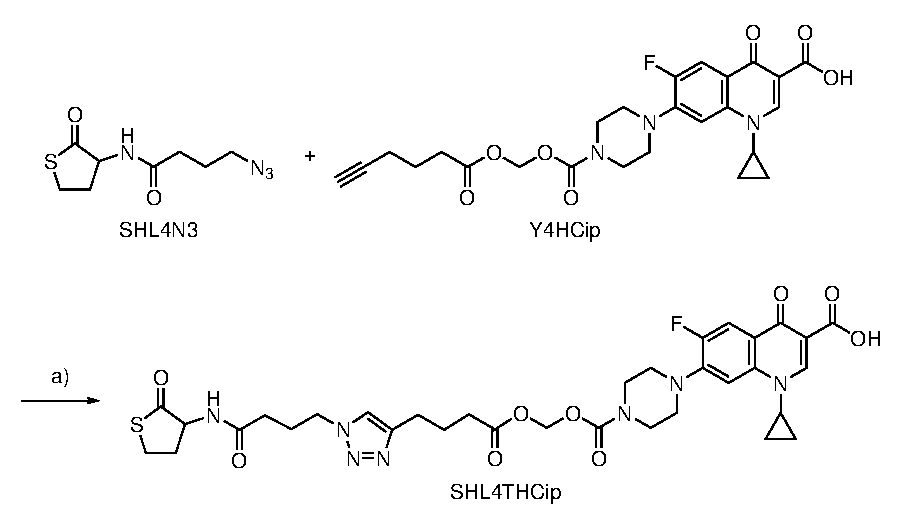
\includegraphics[scale=1]{SHL4THCip_synth}
		\caption{
			Synthesis of the cleavable HCTL-Cip triazole conjugate \compound{cmpd:SHL4THCip}.
			a) CuI, DIPEA, \ce{CH2Cl2}, r.t., 3 h, 5.0 \%.
			\label{sch:SHL4THCip_synth}}
	\end{center}
\end{scheme}